%Ukazka zaverecne zpravy
%Posledni zmena 02/2017, Martin Cadik

\documentclass[11pt,a4paper,oneside]{article}
\usepackage[utf8]{inputenc}
%\usepackage{a4wide}
\usepackage{amsmath}
\usepackage{mathtools}
\usepackage{url}
\usepackage{algorithm}
\usepackage[noend]{algpseudocode}
\floatname{algorithm}{Alg.} 
\DeclarePairedDelimiter\ceil{\lceil}{\rceil}
\DeclarePairedDelimiter\floor{\lfloor}{\rfloor}

\usepackage{ifpdf}
\ifpdf
\usepackage[pdftex]{graphicx}
\DeclareGraphicsExtensions{.pdf,.png,.gif,.jpg}
\else
\usepackage[final]{graphicx}
\DeclareGraphicsExtensions{.eps,.png,.gif,.jpg}
\fi 

\begin{document}
	%Uvodni stranka
	\thispagestyle{empty}
	\begin{center}
	\vspace*{60mm}
	{Semestrální projekt xx -- závěrečná zpráva }\\
	\smallskip
	{\Large\bf Převod barevného obrazu na šedotónový}\\
	\smallskip
	{\it Ján Brída, \url{xbrida01@stud.fit.vutbr.cz}}\\
	\vfill
	{\bf Vedoucí práce:} {\it doc. Ing. Martin Čadík, Ph.D., \url{cadik@fit.vutbr.cz}} 
	\hfill {Květen 2017}

	\end{center}
	\newpage

	%Vlastni zprava
	\section{Úvod}
	Tento semestrální projekt se zaobírá problematikou transformace barevného obrazu
	na šedotónový. Černo-bílé fotografie se stále běžně objevují v~mnohých
	sférách vizuální prezentace, avšak~problémem šedotónové konverze bývá zachování
	detailů, především v~izoluminantních oblastech. To znehodnocuje celkový
	dojem a~sňižuje schopnost pochopit obsah obrazu.

	Bylo navrženo množství metod, kterými jsou barevné obrazy převáděny do šedotónové podoby.
	Typicky jsou rozděleny na globální a~lokální, podle toho, zda-li jsou zkoumány závislosti
	v~obraze. Prvně jmenované bývají často dostatečně rychlé, neposkytují však vždy vizuálne
	věrohodnou reprezentaci vzhledem ke vstupu. Lokální techniky se typicky snaží brát v~úvahu
	barevné změny v~oblastech a~uspůsobit podle nich výpočet luminance. Některé takovéto
	algoritmy pracují v~gradientní doméně.

	Takovýmto algoritmem je i~transformace podle experimentů s~barevným systémem
	zvaným Coloroid~\cite{cadik07color_to_gray}. Podobá se metodě~\cite{gooch2005color2gray},
	která iterativně minimalizuje chybu objektivní funkce, podle lokálních kontrastů mezi pixely, na základě
	transformace do CIE L*a*b*. Ta se snaží zachovat detaily použitím rozdílů luminance
	nebo chrominance (maximum) mezi pixely, dochází ale naneštěstí k~nekonzistencím.
	Navíc není algoritmus automaticky adaptabilní, protože vyžaduje nastavení
	trojice parametrů ovlivňující výslednou transformaci.

	\section{Šedotónová transformace}
	Jedná se o~redukci alespoň 3 barevných složek (např. RGB) na 1D data.
	Jak bylo zmíněno, výzvou takovéhoto převodu je zachovat ekvivalentní
	přechody v~novém obraze, aby byl výsledek percepčně blízký vstupu.

	\subsection{Coloroid}
	Barevný systém Coloroid byl vytvořen pro popsání spojitého barevného prostoru,
	který je esteticky uniformní protože dokáže definovat harmonické vztahy mezi barvami,
	jelikož sousedící barvy jsou určeny stejně velkými celočíselnými intervaly.
	Spojitost barevného prostoru Coloroidu poskytuje možnost jednoznačne určit
	vztahy mezi barvami v~jiných barevných systémech. Coloroid vynalezli v~60.-80. letech
	minulého staletí v~Budapešti na základě experimentů při sledování barev pozorovatelem,
	celkově bylo těchto jednotlivců až $70\,000$.

	Barvy jsou v~tomto 3D prostoru definovány pomocí HSL (\emph{hue}, \emph{saturation},
	\emph{luminance}) komponent (obrázek~\ref{fig:coloroid}).
	Coloroid reprezentuje válec, kde angulární souřadnice
	(A) určuje odstín, nasycení definuje radiální souřadnice (T) a~na vertikální ose (V)
	se pohybuje svítivost barvy. Důležitou informací je, že s~nulovou saturací je barva
	reprezentována v~šedotónové oblasti. 48 základních barev  v~základni kužele
	představuje vztah k~CIE 1931 barevnému gamutua~nejvíce nasycené mají hodnoty na obvodu tohoto kruhu.

	V~práci~\cite{cadik07color_to_gray} je Coloroid využit pro převod na percepčně blízký šedotónový výsledek
	vstupního obrazu. Autoři provedli sledování několika barev, kde náhle jedna z~nich byla
	nahrazena za nesaturovaný vzorek. Pozorovatel po změně zhodnotil uniformitu vnímání v~krátkém
	čase (aby oko nemělo čas se přispůsobit). Na základě těchto experimentů došlo na
	substituci šedotónových vzorků do vygenerovaných posloupností s~fixními A, V komponentami
	a~postupně rostoucí saturací. Výsledkem byl poznatek, že nedochází k~monotónní diferenci mezi
	těmito vzorky v~šedotónové oblasti.

	Byla vytvořena matice $7 \times 7$ šedotónových změn mezi 7 vybranými odstíny (zástupci 7 skupin
	základních barev Coloroidu). Na diagonále se vyskytují nuly a~je anti-symetrická, viz
	jak byly hodnoty naměřeny~\cite{cadik07color_to_gray}. Tato matice je základním stavebním prvkem pro převodovou
	rovnici na šedotónovou podobu. Zbylé barvy získají své diference bilineární interpolací.

	\begin{figure}[htb]
		\centering
		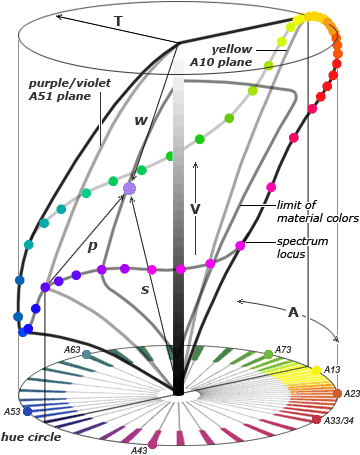
\includegraphics[scale=0.5]{fig/Coloroid.png}
		\caption{Model barevného prostoru Coloroid.} 
		\label{fig:coloroid}
	\end{figure}

	\subsection{Rovnice pro šedotónovou transformaci}
	Hledanou veličinou je gradient, popisující rozdíl mezi dvěmi Coloroid
	barvami $(A_1, T_1, V_1)$, $(A_2, T_2, V_2)$ a~je vypočten podle
	rovnice~\eqref{eq:grad}. Ta obsahuje termy diferencí luminance
	(rovnice~\eqref{eq:lum}), saturace (rovnice~\eqref{eq:sat}) a~odstínu
	(rovnice~\eqref{eq:hue}), postupně odvozeny na základě~tabulky změn
	pro 7 barevných skupin.

	\begin{equation}
		\Delta_{1, 2} = dL(L_1, L_2) + S(A_1, T_1, V_1, A_2, T_2, V_2) + h(A_1, T_1, A_2, T_2)
		\label{eq:grad}
	\end{equation}

	Gradient odstínu dvou barev $A_1$, $A_2$ je vypočten jako
	\begin{equation}
		h(A_1, T_1, A_2, T_2) = w_h \cdot H(A_1, A_2) \cdot \sqrt{u(T_{1rel}) \cdot u(T_{2rel})},
		\label{eq:hue}
	\end{equation}
	kde $T_{rel}$ je relativní saturace pro každou rovinu odstínů v~každé úrovni luminance.
	Term $u(x)$, kde $x = 2 \cdot T_{rel}$, je definován jako $u(x) = 0.5 \cdot x$, pokud $x < 0.5$
	a~$u(x) = \sqrt{x} - 0.5$ jinak.

	Určení šedotónové změny pro korespondující saturaci závisí na
	\begin{equation}
		S(A_1, T_1, V_1, A_2, T_2, V_2) = w_s \cdot \left[S(A_2, T_2, V_2) - S(A_1, T_1, V_1)\right]
		\label{eq:sat}
	\end{equation}
	a~pro luminanci
	\begin{equation}
		dL(L_1, L_2) = L_2 - L_1,
		\label{eq:lum}
	\end{equation}
	jak je podrobněji rozebráno odvození těchto rovnic v~\cite{cadik07color_to_gray}.

	\subsection{Výpočet na základě gradientního pole}
	Obdržený nekonzistentní gradientní obraz je následně stabilizován pomocí speciální metody, užívající
	ortogonální projekci pro nalezení nejbližšího konzistentního gradientního pole. Výsledek
	tohoto procesu je nakonec zpracován integrací podle navštíveného gradientu~\cite{cadik07color_to_gray}.

	Hlavní myšlenkou korekce gradientního pole $\mathbf{g}$ je určit chybu $E_{(i, j)}$
	jednotlivých elementárních smyček všech pixelů. Konzistentní gradientní pole po
	této úpravě musí splňovat rovnost
	$$
		\mathbf{g}_{(i + 1, j), x} + \mathbf{g}_{(i, j), y} =
		\mathbf{g}_{(i, j), x} + \mathbf{g}_{(i, j + i), y}.
	$$

	Algoritmus opakovaně prochází daný obraz a~pro každý pixel spočte $E_{(i, j)}$ podle výše uvedeného
	vztahu. Chyba je pak distribuována, čímž je obdržen nový gradient $\mathbf{g}(i, j)$. Definice
	numerické metody představuje
	\begin{equation}
		\mathbf{g}^{(k + 1)} = \mathbf{g}^{(k)} - \frac{1}{4} \cdot E_{(i, j)} \cdot \mathbf{N}_{(i, j)},
	\end{equation}
	kde $\mathbf{N}_{(i, j)} = (0, \dots, 0, +1, +1, -1, -1, 0, \dots, 0)$ identifikuje $2 \cdot
	N \cdot M$ vektor s~odpovídajícími nenulovými koeficienty pro $\mathbf{g}_{(i,j)}$, kde $N$
	je výška a~$M$ šířka obrazu. $E_{(i, j)}$ postupně konverguje k~nule. V~algoritmu~\ref{alg:correct_grad}
	představuje $1 < \omega < 2$ urychlení konvergence.

	\begin{algorithm}
		\caption{Sekvenční algoritmus korekce gradientního pole $\mathbf{g}$.}
		\label{alg:correct_grad}
		\begin{algorithmic}[1]
			\Function{correct gradient}{$\mathbf{g}$, $\omega$, $\epsilon$}
				\Repeat
					\State $E_{\max} \gets 0$
					\For{$i \in \left\{0, \dots, N\right\}$}
						\For{$j \in \left\{0, \dots, M\right\}$}
							\State $E \gets \mathbf{g}_{(i + 1, j),x } + \mathbf{g}_{(i, j), y} -
									\mathbf{g}_{(i, j), x} - \mathbf{g}_{(i, j + i), y}$

							\If{$|E| > E_{\max}$}
								\State $E_{\max} \gets |E|$
							\EndIf
							
							\State $E \gets \frac{1}{4} \cdot E \cdot \omega$

							\State $\mathbf{g}_{(i, j), x} \gets \mathbf{g}_{(i, j), x} - E$
							\State $\mathbf{g}_{(i, j + 1), y} \gets \mathbf{g}_{(i, j + 1), y} - E$
							\State $\mathbf{g}_{(i + 1, j), x} \gets \mathbf{g}_{(i + 1, j), x} + E$
							\State $\mathbf{g}_{(i, j), y} \gets \mathbf{g}_{(i, j), y} + E$
						\EndFor
					\EndFor
				\Until{$E_{\max} > \epsilon$}
			\EndFunction
		\end{algorithmic}
	\end{algorithm}

	\subsubsection{Optimalizace}
	Výše uvedený algoritmus je cyklickým řešením korekce gradientu jeho elementárních smyček obrazu.
	Urychlení výpočtu pomocí data paralelních algoritmů na grafické kartě rozděluje algoritmus
	na 3~zájmová místa (následující výčet referuje řádky algoritmu~\ref{alg:correct_grad}):
	\begin{enumerate}
		\item \#6: paralelní výpočet chyby $\mathbf{E}_{(i, j)}$ všech elementárních smyček,
		      kde $\mathbf{E}$ je vektor o~velikosti $N \cdot M$,
		\item \#7-8: redukce $\mathbf{E}$ s~asociativním operátorem $\max$ pro získání $E_{\max}$,
		\item \#10-13: aby nedocházelo k~čtecím/zápisovým~datovým konfliktů, jsou jednotlivé
		      přiřazení výsledků provedeny paralelně samostatně.
	\end{enumerate}

	Je možné vytvořit i~efektivnejší modifikaci této korekce výběrem upravované elementární smyčky
	na základě maximální chyby $E_{\max}$ v~jedné iteraci algoritmu~\cite{cadik07color_to_gray}.
	Určení elementární smyčky s~$E_{\max}$ v~paralelním prostředí může být zjednodušeno na nalezení odpovídajícího indexu
	pixelu během redukce $\mathbf{E}$. Index je jednoduše definován pracovním identifikátorem
	výpočtu a~dodatečne vyžaduje $\ceil*{N \cdot M}_{(2 \cdot W)} \div {(2 \cdot W)}$
	paměťového místa pro uchování této informace při rekurzivní redukci, kde $W$ určuje velikost
	pracovní skupiny.

	\section{Implementace}
	Popis implementace a vizualizace jednotlivých fází výpočtu.

	\section{Výsledky}
	Nejdůležitější část -- diskuse výsledků, 
	načtené/vypozorované klady a zápory, operační složitost, ...
	Ukázkové obrázky.

	\subsection{Uživatelská studie}
	Poznatky získané testováním.

	\section{Závěr}

	\bibliographystyle{acm}
	\bibliography{report}
\end{document}
